\documentclass[eng,openany]{mgr}
\usepackage{listings}
\usepackage[english]{babel}
\usepackage{graphicx}
\usepackage{hyperref}
\usepackage{tabularx,colortbl} 
\usepackage{rotating}
\usepackage[utf8]{inputenc} 
\setlength\parindent{24pt}
\usepackage{float}

%tlmgr init-usertree
%sudo apt-get install xzdec
%sudo tlmgr install collection-fontsrecommended



% Default fixed font does not support bold face
\DeclareFixedFont{\ttb}{T1}{txtt}{bx}{n}{12} % for bold
\DeclareFixedFont{\ttm}{T1}{txtt}{m}{n}{12}  % for normal

% Custom colors
\usepackage{color}
\definecolor{deepblue}{rgb}{0,0,0.5}
\definecolor{deepred}{rgb}{0.6,0,0}
\definecolor{deepgreen}{rgb}{0,0.5,0}

\usepackage{listings}

% Python style for highlighting
\newcommand\pythonstyle{\lstset{
language=Python,
basicstyle=\ttm,
otherkeywords={self},             % Add keywords here
keywordstyle=\ttb\color{deepblue},
emph={MyClass,__init__},          % Custom highlighting
emphstyle=\ttb\color{deepred},    % Custom highlighting style
stringstyle=\color{deepgreen},
frame=tb,                         % Any extra options here
showstringspaces=false            % 
}}


% Python environment
\lstnewenvironment{python}[1][]
{
\pythonstyle
\lstset{#1}
}
{}

% Python for external files
\newcommand\pythonexternal[2][]{{
\pythonstyle
\lstinputlisting[#1]{#2}}}

% Python for inline
\newcommand\pythoninline[1]{{\pythonstyle\lstinline!#1!}}

\renewcommand\lstlistlistingname{List of code listings}
\newcommand{\linia}{\rule{\linewidth}{0.4mm}}
\author{Jarosław Szumega 196018}
\title{Translation system based on Multilayer Perceptron: pictures of characters into a Morse alphabet signs.}
\engtitle{}
\supervisor{dr inż. Jacek Mazurkiewicz}
\field{Computer Science}
\specialisation{Internet Enginering}
\date{14.12.2015}
\begin{document}
\maketitle
\tableofcontents
\chapter{Problem description}

Main task is to implement a system to recognize a pictures of characters (assumed that they will be computer's fonts) and then translate them into a Morse codes using some kind of dictionary.\\
Recognition will be performed by using Multilayer Perceptron - form of neural network that besides input and output layer has also one or more hidden layers. Their task is to improve the computations and make entire network more sensitive.
\\\\
\begin{figure}[h]
\centering

\includegraphics[width=0.5\linewidth]{./morse}
\caption{Standard for coding characters in Morse code.}
\label{fig:morse}
\end{figure}
\\
As the figure \ref{fig:morse} presents, the Morse Code is an alphabet with non-fixed word length. Multilayer perceptron should have the fixed number of input neurons. Due to that fact only the characters coded with word of length four were chosen to perform experiments.
\chapter{Solution}
\section{Tools to be used}
For purpose of implementation \textbf{Python} was chosen. It is scripting, high-level language with many scientific libraries. And as a plus it was primely designed to work with UNIX-like systems.\\
Following libraries were used to realize the project:
\begin{itemize}
\item PyBrain - it is a Machine Learning Library for Python. Its modules contain a number of algorithms for neural network and machine learning purposes. In following project it was used to build a neural network and perform supervised learning.
\item Pillow - is still being developed fork of PIL (Python Image Library that is no longer supported). It is similar to Matlab Image Processing Toolbox.\\
Used mainly for reading images and preprocessing purposes for input of neural network.
\end{itemize}
\section{Network design}
The neural network build to realise characters recognition has following structure:
\begin{itemize}
\item 900 neurons in input layer - the number of neurons is a results of using pictures of size 30x30 pixels. Each neuron corresponds to particular pixel.
\item 60 neurons in hidden layer - that layer exists to improve computations and perform transformation inputs to outputs. Hidden layer uses also activation function. e.g. sigmoid or hyperbolic tangent.
The number of neurons is fixed according to often used formula:\\ $hidden_neurons = \sqrt{in\_neurons * out\_neurons}$.
\item 4 neurons in output layer - four signs Morse code characters were chosen, so at the output there is a need to establish four elements.
\end{itemize}
\newpage
\section{Datasets and network training}

For teaching purposes there was prepared eight sets of four-sign characters. Different fonts were chosen in order to keep variety of characters (picture \ref{fig:alphabet}).
\begin{figure}[h]
\centering
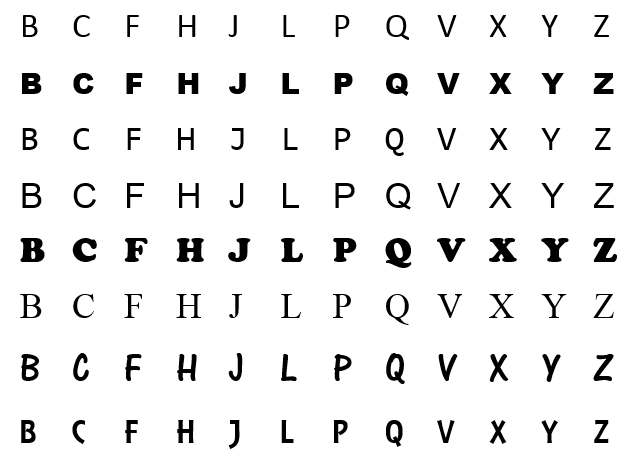
\includegraphics[width=0.7\linewidth]{./alphabet}
\caption{Prepared characters. Version without noise or other distortions.}
\label{fig:alphabet}
\end{figure}
Presented above letters were translated into datasets in \textit{CSV} format. A long vector of zeros and ones (representing white or black, also according to some threshold) was concatenated to correct output. That kind of file was used to train the network.
\\
\\
The neural network was trained using following parameters:
\begin{itemize}
\item learning rate = 0.01, establishes how fast the weight changes during training process.
\item momentum = 0.5, used for preventing network from converging to local minimum.
\item back-propagation as a teaching algorithm.
\end{itemize}
Beside presented above "clean" sets, there are also prepared "noisy" ones. To be more precise - using written for that purpose Python's  script, the pictures with some percentage of noise were generated as well as ones with some blank lines (number of lines also can be passed as an argument).
\begin{figure}[h]
\centering

\includegraphics[width=0.3\linewidth]{./c}
\caption{Examples of broken images.}
\label{fig:c}
\end{figure}
\newpage
\section{Implementation}
Core script for creating structure and proper set-up of designed network:
\\
\begin{python}
#!/usr/bin/python

from pybrain.structure import FeedForwardNetwork
from pybrain.structure import FullConnection
from pybrain.structure import LinearLayer, SigmoidLayer, TanhLayer
from pybrain.tools.xml.networkwriter import NetworkWriter
from pybrain.tools.xml.networkreader import NetworkReader

class MyNet:

	def __init__(self, file='config.xml'):
		self.net = FeedForwardNetwork()
		self.file = file

	def constructNet(self, input, hidden, output): 
		inputLayer = LinearLayer(input)
		hiddenLayer = TanhLayer(hidden)
		outputLayer = LinearLayer(output)

		self.net.addInputModule(inputLayer)
		self.net.addModule(hiddenLayer)
		self.net.addOutputModule(outputLayer)

		conn1 = FullConnection(inputLayer, hiddenLayer)
		conn2 = FullConnection(hiddenLayer, outputLayer)

		self.net.addConnection(conn1)
		self.net.addConnection(conn2)

	def setup(self):
		self.net.sortModules()
	
	def saveToFile(self,file='config.xml'):
		NetworkWriter.writeToFile(self.net, file)

	def loadFromFile(self, file='config.xml'):
		self.net = NetworkReader.readFrom(file)

if __name__ == "__main__":
	network = MyNet()
	network.constructNet(900,60,4)
	network.setup()

	network.saveToFile()
\end{python}
Beside presented core program, there were also written following scripts:
\begin{itemize}
\item train.py - network trainer, that using backpropagation algorithm performed teaching process with given parameters and storing results in xml file,
\item liner.py - performs blanking lines in pictures,
\item noiser.py - adds noise to picture - with some probability the pixel can be randomly set between white and black.
\item setbuilder.py - transforms images in given folder (recursively) into a CSV file,
\item validator.py - perfumes image translation into Morse code and validates the result. A set of images can be given. At the end the statistics of successful operations will be displayed.
\end{itemize}

\chapter{Tests}
Network is build and trained. The learned datasets are well recognized (100\% in any case).\\
The tests were executed using noisy images. But the clue is to compare results between them.
In order to do that, two versions of neural network were prepared: one uses sigmoid as an activation function in hidden layer, the other one - hyperbolic tangent.\\
\\
Presented here results will establish which one is better in case of presented project.\\


\section{Images with noise}
The most common distortion is white noise. To check network beahaviour, the pictures with some noisiness were generated. Then using validator, the tests were performed and statistics gathered
\begin{figure}[h]
\centering
\includegraphics[width=0.7\linewidth]{../szum/szum1}
\caption{Experiment - build dataset with noise = 0.01}
\label{fig:szum1}
\end{figure}

\begin{figure}[H]
\centering
\includegraphics[width=0.7\linewidth]{../szum/szum2}
\caption{Experiment - build dataset with noise = 0.02}
\label{fig:szum2}
\end{figure}

\begin{figure}[H]
\centering
\includegraphics[width=0.7\linewidth]{../szum/szum5}
\caption{Experiment - build dataset with noise = 0.05}
\label{fig:szum3}
\end{figure}

\begin{figure}[H]
\centering
\includegraphics[width=0.7\linewidth]{../szum/szum10}
\caption{Experiment - build dataset with noise = 0.10}
\label{fig:szum4}
\end{figure}
\noindent
\textbf{Results}\\
As the picture presents, in most cases the hyperbolic tangent is better. When sigmoid cannot recognize the letters, the hyperbolic tangent still is doing correctly.
\\
\\
The first letter that is not recognized is 'V'.
\section{Images with missing lines}
That kind of distortion can be noticed e.g. using printer. Some lines can be not covered and we receive white lines. Will the network be able to recognize such a thing?
\begin{figure}[H]
\centering
\includegraphics[width=0.7\linewidth]{../szum/linie1}
\caption{One blank line}
\label{fig:linie1}
\end{figure}
\begin{figure}[H]
\centering
\includegraphics[width=0.7\linewidth]{../szum/linie2}
\caption{Two blank lines}
\label{fig:linie2}
\end{figure}
\begin{figure}[H]
\centering
\includegraphics[width=0.7\linewidth]{../szum/linie3}
\caption{Three lines that interrupts recognition.}
\label{fig:linie3}
\end{figure}
\begin{figure}[H]
\centering
\includegraphics[width=0.7\linewidth]{../szum/linie4}
\caption{Four lines - algorithm overloading.}
\label{fig:linie4}
\end{figure}
\noindent
\textbf{Results}\\
\\
As in the previous test - also here the tangent gets proper results more often, but still there are letters when the sygmoid is simply better.\\
Tangent can recognize most of weakly-noised images.

\chapter{Extras}
Beside implementing neural network and performing tests, also the visual effect can be shown.\\
\\
Using Raspberry Pi \ref, there was implemented simple script that takes Morse codes as parameter and using LED transmitts light signals.
\begin{figure}[h]
\centering
\includegraphics[width=0.7\linewidth]{./zdj}
\caption{Raspberry PI model B+.}
\label{fig:zdj}
\end{figure}

\begin{python}

#!/usr/bin/python
import RPi.GPIO as GPIO
import time
import sys

PIN = 7
dot_length = 0.3
dash_length = dot_length*3
pause = dot_length

def blink(timer):
	
	GPIO.output(PIN, True) 
	time.sleep(timer)
	GPIO.output(PIN, False) 
	time.sleep(pause)

def dot():
	print 'dot'
	blink(dot_length)
	
def dash():
	print 'dash'
	blink(dash_length)
	
def control(arr):
	for e in arr:
		if e == '0':
			dot()
		if e == '1':
			dash()

def setup():
	GPIO.setmode(GPIO.BOARD)
	GPIO.setup(PIN, GPIO.OUT)	
	GPIO.setwarnings(False)

def process():
	list = [sys.argv[1],sys.argv[2],sys.argv[3],sys.argv[4]]
	return list	
	
def main():
	
	setup()	
	if len(sys.argv)==5:
		code = process()
		control(code)

main()

\end{python}
It can be connected to neural network (e.g. using tcp messages in ZMQ protocol).\\
That way, there was obtained practical system that not only recognizes the characters, but after translating them into Morse codes, it can also send visual signals.
\chapter{Conclusions}
Despite well-known structure of neural network type, solutions has to be independently decided.\\Even small things such as hidden layer activation function can has a huge impact on results.
\\
\\
In presented translation system had better results using hyperbolic tangent. And it was not so well trained as sygmoid, but still achieved better.
\\
Training can last long in order to achieve proper results (the longest round of 10 000 epochs took almost 8 hours).
\\
The neural network can be applied in simple projects. The example can be presented here Morse transmitter based on RPi. It does not require much work, but shows practical approach and possibility of application.
\\
\\
\textbf{Final remarks}\\\\
To build working network and achieve good results the tests should be done. They can help to establish if activation function is properly set or not.
\\
Time should also be given to train the network. It is process that will determine the error of network, so it is worth to spend some time on it.

\begin{thebibliography}{\bibliography{}}
\bibitem SSoftcomputing course slides, Jacek Mazurkiewicz
\bibitem ppyBrain documentation and tutorial, CogBotLab \& Idsia
\bibitem AArtificial Neural Networks, Wikibooks
\bibitem PPILLOW - fork od Python Imaging Library documentation.
\end{thebibliography}
\end{document}
